% !TEX encoding = UTF-8 Unicode
\documentclass[a4paper,12pt]{article}
\usepackage{polski}
\usepackage[utf8]{inputenc}
\usepackage{graphicx}
\usepackage{float}
\usepackage{rotating}
\usepackage{caption}
\usepackage{subcaption}
\usepackage{pdfpages}
\usepackage{ucs}
\usepackage{amsmath}
\usepackage{amsfonts}
\usepackage{amssymb}
\usepackage{ucs}
\usepackage{epstopdf}
\usepackage{epsfig}
\usepackage{url}


\begin{document}
% Strona tytułowa
\begin{titlepage}
\begin{center}
\vspace*{1cm}
{ \Large \textbf{ Raport }}\\[1cm]

%{ \Large \textsc{\\ robota mobilnego} }\\[2cm]

{ \Large Projekt specjalnościowy ARR \\
\textbf{Stanowisko do badania systemu sensorycznego cybernetycznej dłoni}}\\
Semestr letni 2016/2017\\[2cm]

\Large{
\textbf{Zespół:}}\\
\large {Artur Błażejewski, 200541\\
Dawid Chechelski, 197002\\
Paweł Jachimowski, 200355\\
Krzysztof Kwieciński, 200418\\
Witold Lipieta, 200415}

\vfill
\Large
Politechnika Wrocławska\\
\large
Wydział Elektroniki\\
Automatyka i Robotyka\\
ARR
\end{center}
\end{titlepage}


	\section{Komponenty układu}
		\subsection{Cybernetyczna proteza dłoni - Grzegorz Wiśniewski}
			W projekcie czujniki zostały umieszczone na protezie skonstruowanej przez Grzegorza Wiśniewskiego \cite{Reka}.
		\subsection{Czujniki}
			W projekcie zostały wykorzystane moduły czujników stworzone przez Mariusza Głębockiego \cite{Moduly}.
			
			W modułach zostały zastosowane czujniki MPL115A2 \cite{MPL112A2}.
			
		\subsection{Płytka}
			
			\begin{figure}[H]
		     	 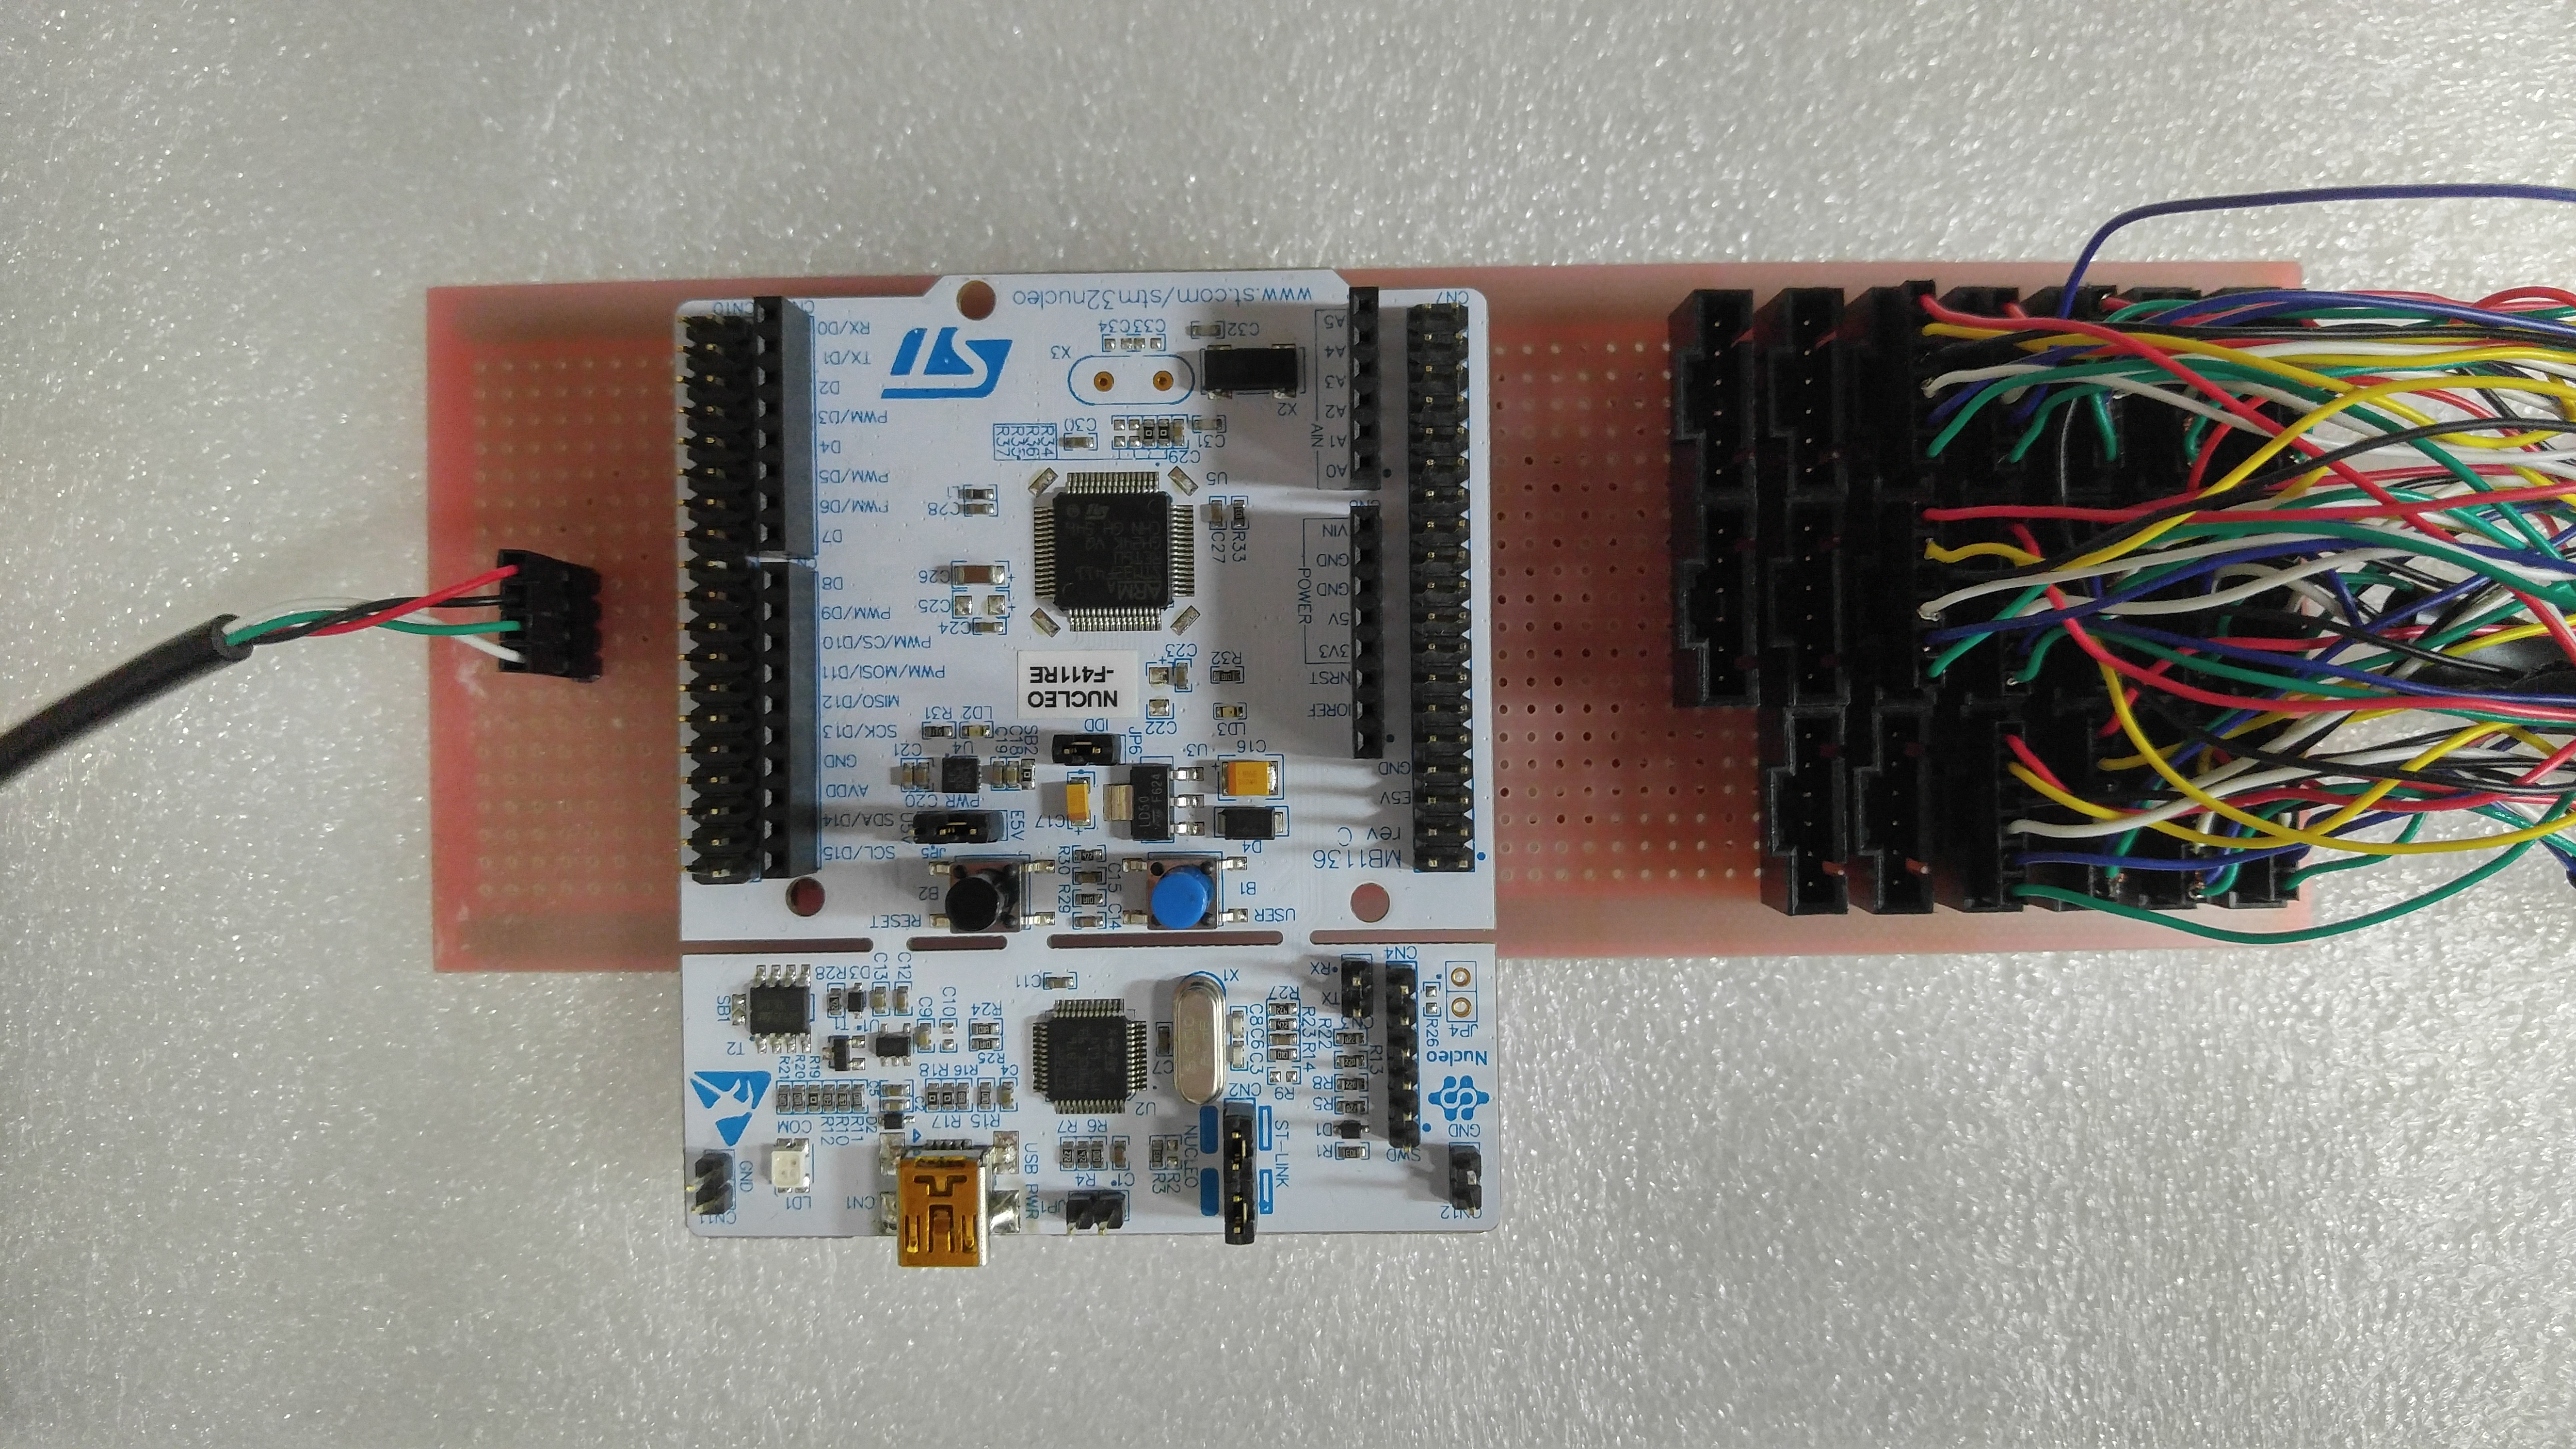
\includegraphics[width=1\textwidth]{obrazy/plytka.jpg}
			\end{figure}
		
			\subsubsection{Płytka}
				W projekcie została użyta uniwersalna płytka o wymiarach 17x6,5~cm, na której zostało umieszczone 20 złącz pod czujniki oraz złącze pod komunikację UART i~Nucleo. 
						
			\subsubsection{Moduł nucleo}
				Ze względu na potrzebną ilość portów komunikacji I$^2$C wybrano moduł STM32 NUCLEO-F411RE
			
	\section{Wykonanie projektu}		
		\subsection{Komunikacja}
			\subsubsection{Czujniki}		
				Czujniki z~modułem Nucleo wykorzystują do połączenia komunikację I$^2$C. Każdy czujnik jest odpytywany osobno, a~następnie zebrane dane są przesyłane do komputera. 
			\subsubsection{Przesyłanie danych do komputera}
			Dane przesyłane są w~postaci ośmiobajtowej ramki. Pojedyncza wiadomość zawiera informacje o~ciśnieniu, temperaturze oraz identyfikatorze czujnika, a~także bajt startu i~sumy kontrolnej. %TODO -> to chyba całe do zmiany
			\subsubsection{Komputer}
				Połączenie ręki z~komputerem zostało opracowane z~wykorzystaniem komunikacji UART. W tym celu skonfigurowano odpowiednie wyprowadzenia z~mikrokontrolera na płytce Nucleo. Od strony komputera użyto przejściówki RS-232 na USB. Prędkość komunikacji ustawiono na 115200 bps, co wystarcza do szybkiego przesyłania danych z~czujników.	
		\subsection{Software}
			\subsubsection{Nucleo}
				Program został napisany w języku C i~źródła wraz z~komentarzem są załączone do raportu w~osobnych plikach.
			\subsubsection{Wizualizacja}
				Część wizualizacyjna została napisana w~języku C++ i~bibliotekach Qt. Źródła projektu wraz z~niezbędną dokumentacją są załączone w~osobnych plikach.
		\subsection{Rozmieszczenie czujników na ręce}
		Czujniki zostały rozmieszczone w następujący sposób:
		\begin{itemize}
			\item na kciuku zostały umieszczone dwa moduły: jeden z~trzema czujnikami, a~drugi z~dwoma,
			\item na palcu wskazującym umieszczono dwa moduły: jeden z~trzema czujnikami, a~drugi z~jednym czujnikiem,
			\item na palcu środkowym znajdują się dwa moduły: jeden z~trzema czujnikami, a~drugi z dwoma.
		\end{itemize}
		
		\begin{figure}[H]
		     	 \includegraphics[width=1\textwidth]{obrazy/dlon.jpg}
			\end{figure}
			
			Rozmieszczenie czujników było oparte na wcześniejszym projekcie oraz brakiem odpowiedniej liczby sprawnych sensorów. Moduły zostały zamocowane do konstrukcji metalowej za pomocą kleju.
		

	\section{Rezultaty projektu}	
	
	\begin{figure}[H]
		     	 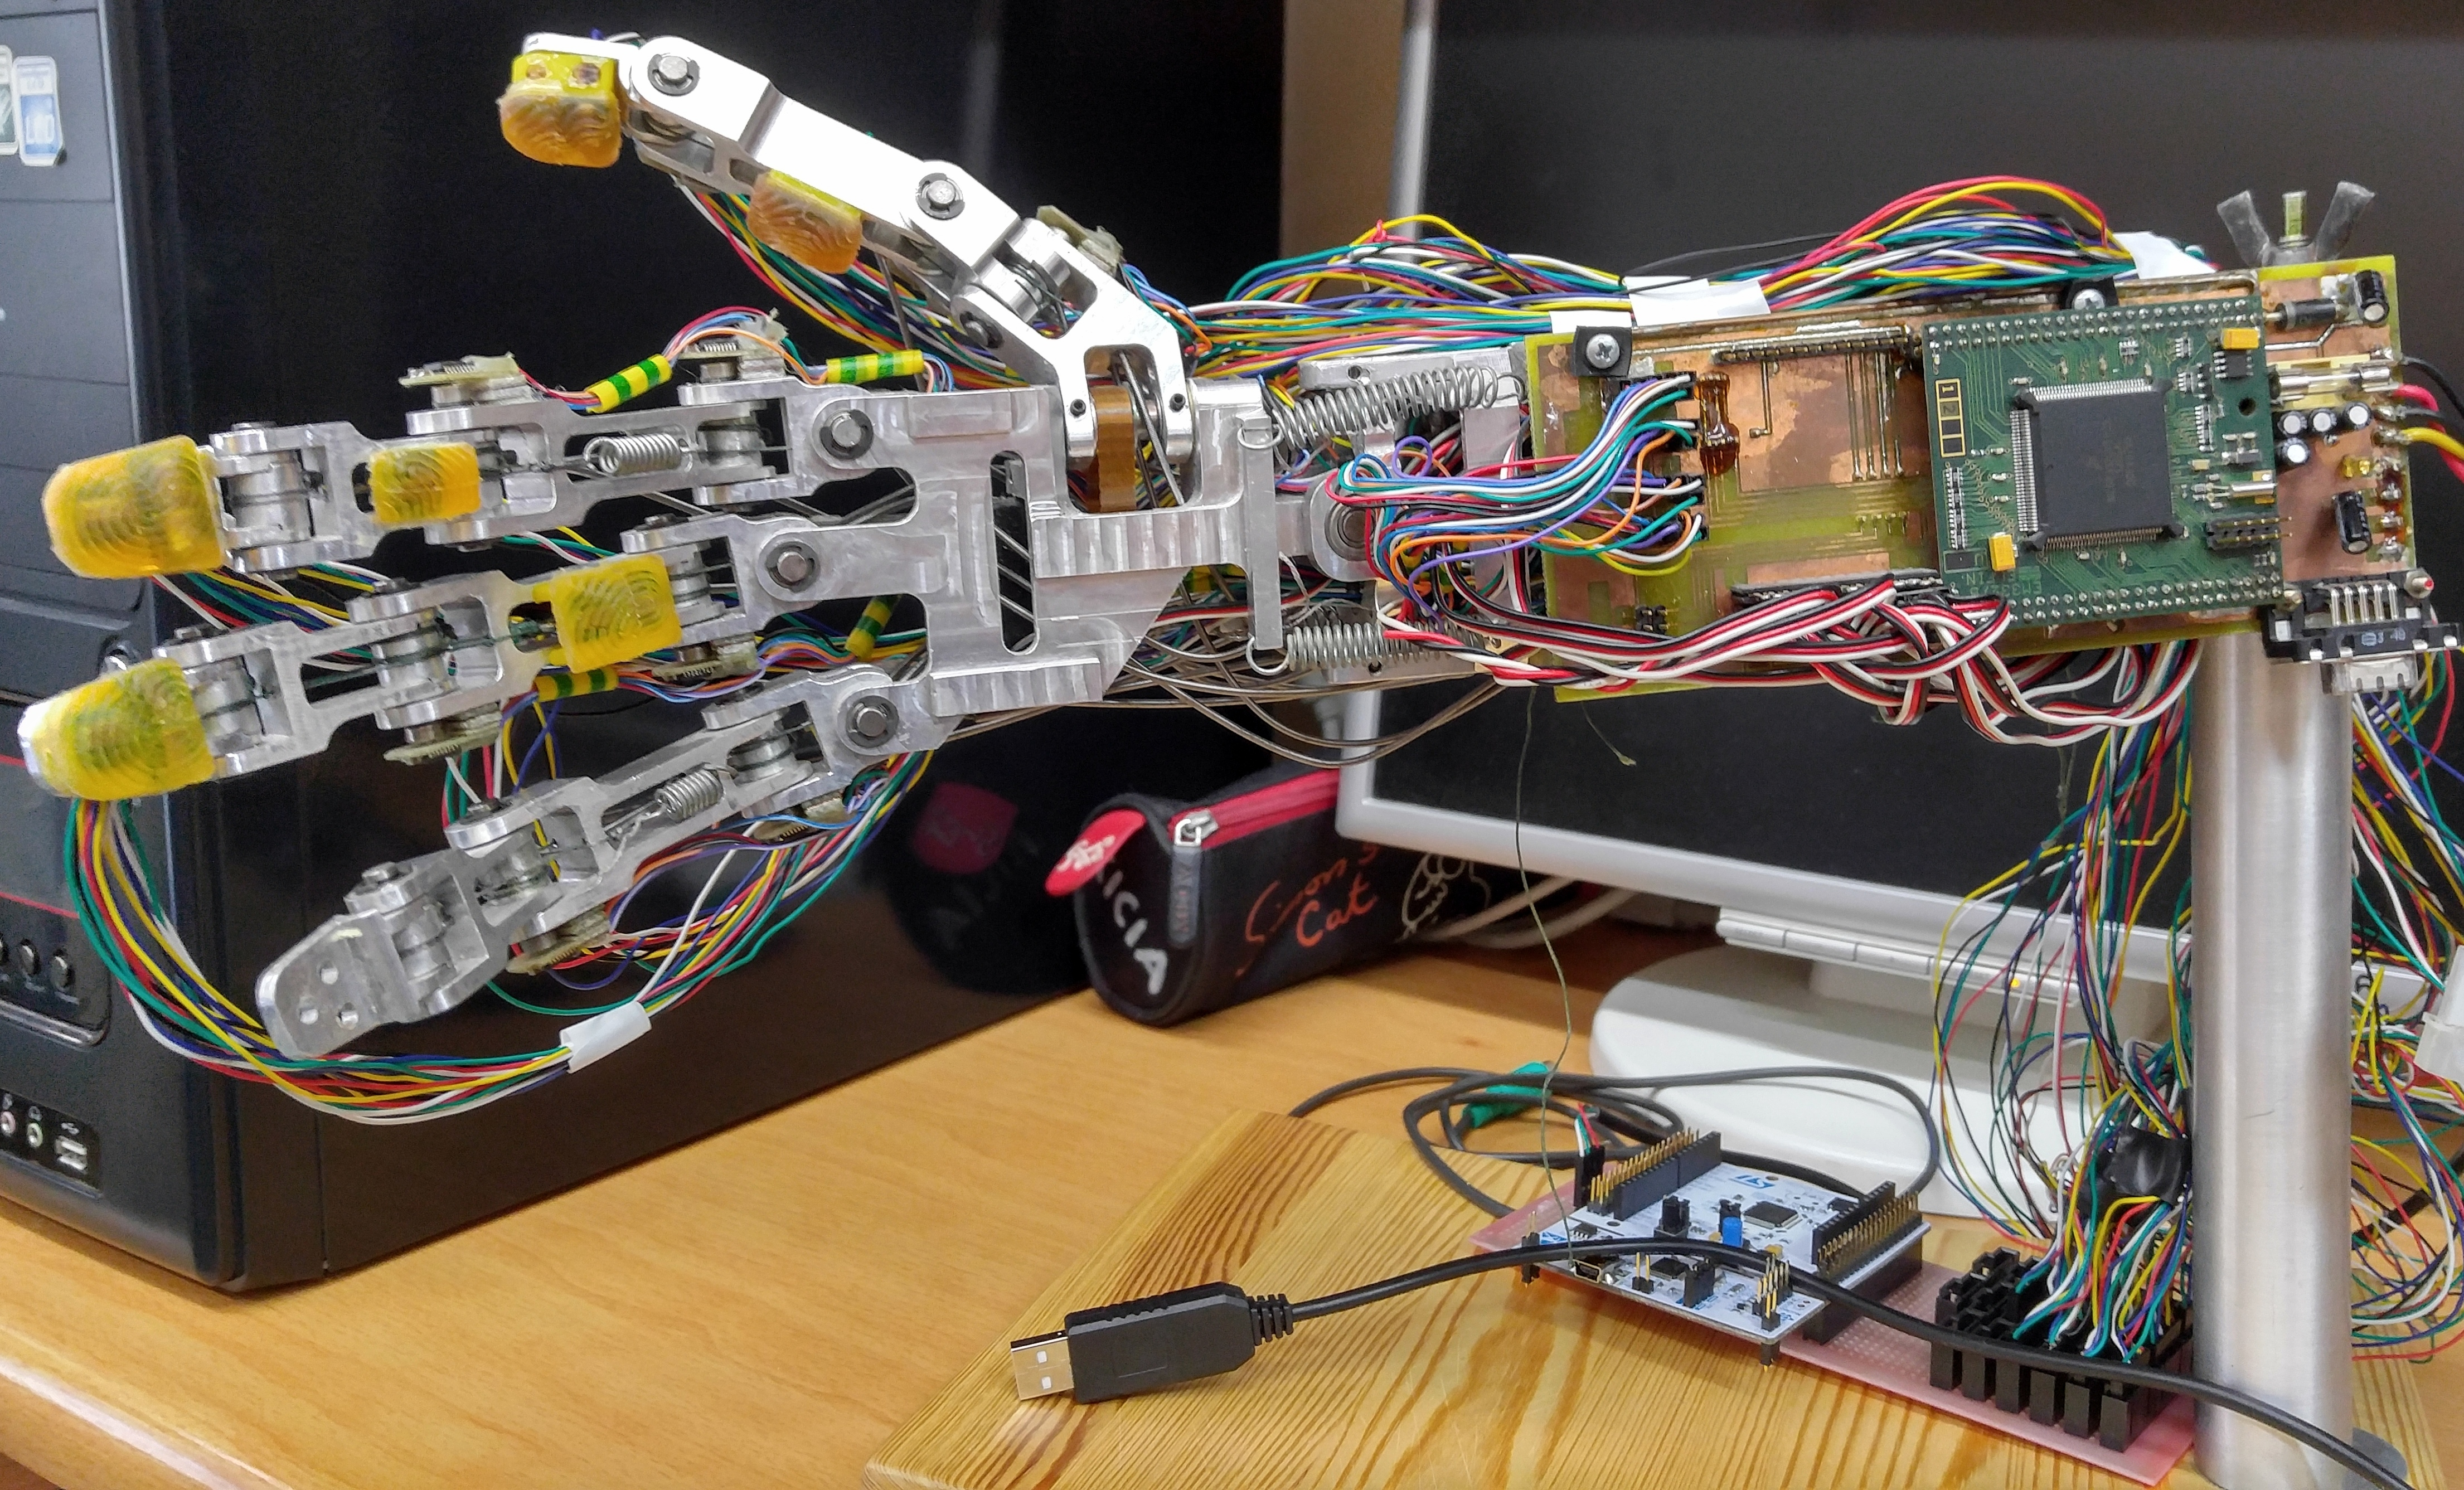
\includegraphics[width=1\textwidth]{obrazy/reka.jpg}
			\end{figure}
	
	W wyniku projektu zostały podłączone i~zamocowane moduły do zbierania informacji o~nacisku i~temperaturze dotykanych przedmiotów. Układ został podłączony do płytki Nucleo i~dalej za pomocą komunikacji UART dane z~czujników są przesyłane do komputera. Na potrzeby zobrazowania działania modułów został wykonany program wizualizujący ich działanie. 
Po wysłaniu DOPISZCIE KTO SIĘ ZNA CO TO JEST -> jak się wyśle coś do procesora to zwraca jakieś coefisienty z charakterystyką czujników.	%TODO koefiszienty to Witka domena, w koncu wykorzystalismy ,,magiczne współczynniki Jachimowskiego'', ale nie wiem, czy o tym warto wspominać ;)
Poniżej przedstawiony jest przykładowy efekt wizualizacji:
	
	\begin{figure}[H]
		     	 \includegraphics[width=1\textwidth]{obrazy/wizualizacja.png}
			\end{figure}
			
	\section{Wnioski i perspektywy rozwoju}
		Główną trudność w~projekcie stanowiły moduły czujników. Przy projektowaniu i~wykonaniu zostało popełnione kilka istotnych błędów. Na płytkach zostały na stałe wlutowane rezystory podciągające, co spowodowało, że nie można było podłączyć wszystkich czujników do jednej linii. Problem ten został częściowo naprawiony poprzez zastosowanie procesora z~trzema portami komunikacji I$^2$C.
		
		 Kolejnym niedopatrzeniem było wyprowadzanie zbyt dużej ilości przewodów. Możliwe byłoby zmniejszenie ich liczby poprzez połączenie masy i~zasilania już na modułach oraz zastosowanie czujników ze zmiennym adresem. Dzięki takim operacją zamiast wyprowadzenia sześciu przewodów z~czujnika, liczba przewodów byłaby zredukowana do sześciu. Dodatkowo pozwoliłoby to na połączenie przewodów już na dłoni i~ostatecznie poprowadzenie sześciu przewodów z~całego układu modułów.
		
		Płytka została przygotowane pod większą ilość czujników i~podłączając kolejne należało by jedynie zmodyfikować kod programu o~sprawdzanie kolejnych czujników.
	
	\section{Bibliografia}
\begin{thebibliography}{99}

\bibitem{Reka} Cebernetyczna proteza dłoni - system mechaniczny oraz sensoryka i sterowanie,
\textit {Grzegorz Wiśniewski, Wrocław 2010}

\bibitem{Moduly} Sensor dotyku i poślizgu dla wykrywania interakcji chwytaka robotycznego z uchwyconym przedmiotem.,
\textit {Mariusz Głębocki, Wrocław 2016}

\bibitem{MPL112A2} MPL115A2,
\textit {$http://www.nxp.com/assets/documents/data/en/data-sheets/MPL115A2.pdf.$ Dostęp z dnia: 2017-01-14.}






\end{thebibliography}
	
	
\end{document}
